\section{Ray Tracing for Exascale}

When designing our ray tracer for exascale we focused on two key aspects, producing a task based application with an emphasis on avoiding communication.  For simplicity we consider only ray tracing scenes without reflection or refraction, although our proposed algorithm can be extended to handle either in the future.  Our algorithm uses a simple voxel decomposition to split the work required to trace a scene.  Primary camera rays are then sent into the system and propagating through the domain. As secondary rays introduce most of the uncertainty in the amount of communication necessary in a ray tracing algorithm, we introduce a pre-processing technique that distributes light information to each voxel prior to tracing the scene.  This allows the ray tracing step within each voxel to be completely independent of the data in the rest of the domain.  Using this algorithm we can predict an upper bound on the amount of communication necessary (a scene that contains no data), and extrapolate from there rough estimates on how our algorithm might perform on an exascale system.

\subsection{Implementation}

We chose to implement our ray tracer using Intel’s implementation of CnC which is built on top of their Thread Building Blocks (TBB) library as it has the potential to run on today’s systems as well as next generation exascale architecture.  Figure \ref{fig:cnc} shows the proposed CnC graph for our distributed ray tracer. Data collections, step collections and the dependencies between them are represented in the graph. The tags corresponding to each collection are also shown within the graph node. The control collection for the proposed model is static for all steps and defined in an initialization step. The graph begins execution when the object, lights, and camera data are provided, and terminates when it produces an image.

\subsection{Tags}

The tags are different for many of the data and step collections but share common elements.  FRAME refers to one specific frame in the case of an animation.  INSTANCE refers to the current iteration. I, J, K are iterators over spatial data.

\subsection{Data Collections}

OBJECT contains input data for the scene from the environment.  It is in the form of .obj.  DECOMPOSE\_DOMAIN splits this data into voxels and produces VOXEL\_OBJECT, object data for a given voxel.  Triangles that span multiple voxels are duplicated.  The LIGHTS data collection contains data pertaining to any light sources.  VOXEL\_LIGHT contains the same information as LIGHTS plus a traced light mesh for each wall of a voxel.  CAMERA contains the location and direction of the camera.  RAY\_PACKET contains all the rays that intersect a voxel wall for a given wall and iteration.  IMAGE contains the final image data.

\subsection{Step Collections}

\subsubsection{Decompose Domain}

DECOMPOSE\_DOMAIN takes the data to be traced as input and produces subsets of that data based on voxel decomposition.  As load balancing is not a concern a fast uniformly spaced geometric distribution is sufficient.  The number of voxels produced is set at runtime and should be more than the number of nodes available.

\subsubsection{Distribute Lights}

In order to reduce communication of secondary rays, DISTRIBUTE\_LIGHTS lights is responsible for distributing light information to each voxel.  This guarantees each voxel will only need to communicate with its direct neighbors.  The light information produced for each voxel contains the original light sources as well as a light source mesh for each light and each wall of the voxel.  The mesh is produced by tracing rays from each light source to uniformly spaced points along a voxel wall, see Figure \ref{fig:light}.  Where the rays intersect the wall, new point or directional light sources are created.  If the ray is blocked, the node in the light mesh is tagged as in shadow.

\begin{figure}[!htb]
\centering
\begin{subfigure}{.49\columnwidth}
 \centering
  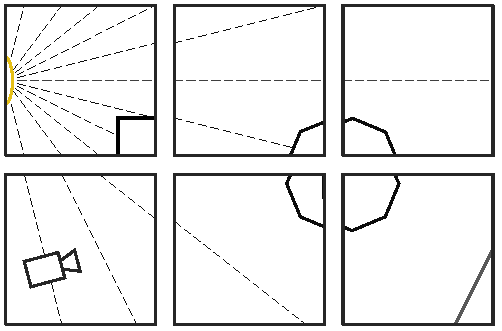
\includegraphics[width=.98\columnwidth]{drawings/Lights1.pdf}
  \caption{Initial light rays}
\end{subfigure}
\begin{subfigure}{.49\columnwidth}
 \centering
  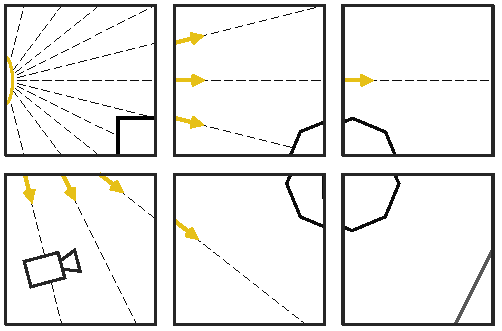
\includegraphics[width=.98\columnwidth]{drawings/Lights2.pdf}
  \caption{Point light sources}
\end{subfigure}
\caption{Light Ray Distribution}
\label{fig:light}
\end{figure}

\subsubsection{Distribute Rays}

DISTRIBUTE\_RAYS is responsible for sending each voxel its first iteration of ray information.  This is an empty set of data for all voxels except the voxel containing the camera if the camera is positioned within the domain.  If the camera is outside the domain, multiple voxels may receive data.

\subsubsection{Trace Voxel}

TRACE\_VOXEL is the heart of the application. This step executes multiple times for each voxel, depending on the size of the domain.  Each time TRACE\_VOXEL executes, it consumes ray packets from each of its neighbors. It then traces the rays over its subset of the domain. If a ray intersects with an object, secondary rays from each light source are considered if the corresponding point or directional light source from the voxels light mesh is not in shadow. Rays that do not intersect objects within the voxels and reach the voxels walls are collected and passed to the corresponding neighbor on the next iteration. See figure \ref{fig:trace}.  Because we are not considering reflection or refraction, we know the maximum amount of times we will have to communicate a single ray across voxel borders in the worst case is proportional to domain size.  This allows us to prescribe the correct number of instances of TRACE\_VOXEL in an initialization step.  For the example in figure \ref{fig:trace} that maximum is 3.  As each CnC step instance will eventually be executed on a single node of a cluster we plan to integrating with Embree, Intel’s ray tracing kernel, in order to optimize per node performance.

\begin{figure}[!htb]
\centering
\begin{subfigure}{.49\columnwidth}
 \centering
  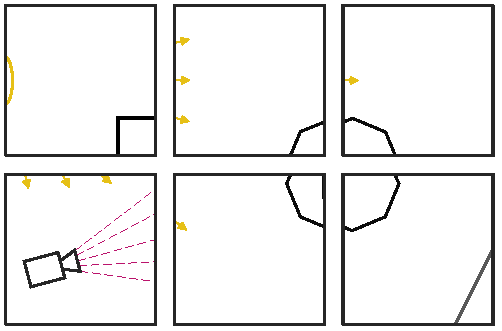
\includegraphics[width=.98\columnwidth]{drawings/Trace1.pdf}
  \caption{Distribute rays}
\end{subfigure}
\begin{subfigure}{.49\columnwidth}
 \centering
  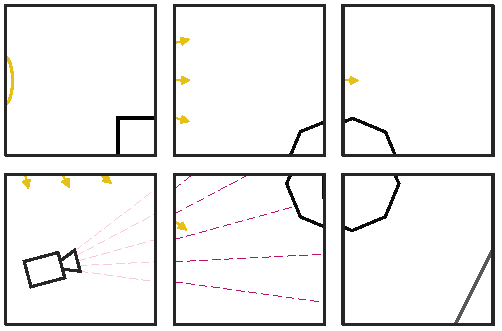
\includegraphics[width=.98\columnwidth]{drawings/Trace2.pdf}
  \caption{Trace voxel; ray step 1}
\end{subfigure}
\begin{subfigure}{.49\columnwidth}
 \centering
  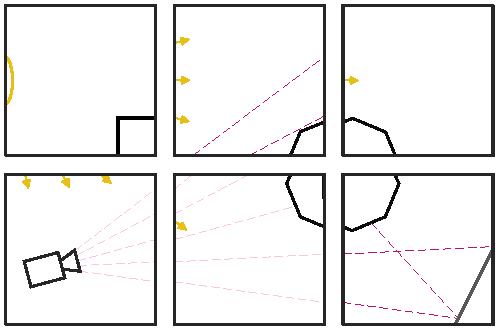
\includegraphics[width=.98\columnwidth]{drawings/Trace3.pdf}
  \caption{Trace voxel; ray step 2}
\end{subfigure}
\begin{subfigure}{.49\columnwidth}
 \centering
  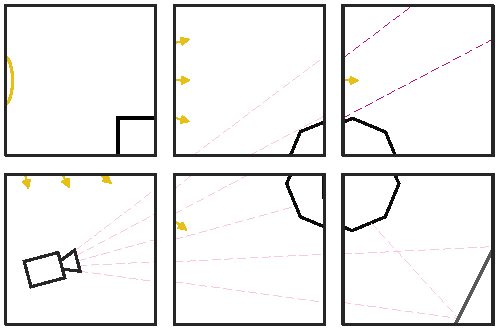
\includegraphics[width=.98\columnwidth]{drawings/Trace4.pdf}
  \caption{Trace voxel; ray step 3}
\end{subfigure}
\caption{Trace Voxel}
\label{fig:trace}
\end{figure}

\subsubsection{Produce Image}
When all step instances of TRACE\_VOXEL have completed, the final set of ray packets is produced.  Each ray in that packet contains the information necessary to produce the final image; merging these is the responsibility of the PRODUCE\_IMAGE step.  

\subsection{Textual CnC Graph File}
To give a more concrete example of how the CnC graph file is implemented, we are including a simplified version the textual representation of TRACE\_VOXEL.  In addition to the step declaration, the code includes the SCENE and RAY\_PACKET data collections as well as the control dependencies from the environment for TRACE\_VOXEL. \\

% Code..
\begin{lstlisting}[language=c,basicstyle=\tiny]
/******************************************************************************
//* Item collection declarations */

// scene data for each voxel, produced by decompose_domain
[ scene_data *scene : frame, i, j, k ];

// ray data passed to neighbors, produced by camera and trace_voxel
[ ray_packet *rays : frame, ray_step, neighbor, i, j, k ];

/******************************************************************************
//* CnC steps */

( trace_voxel : frame, ray_step, i, j, k )
<- [ scene: frame, i, j, k],
   [ rays : frame, ray_step  , 0, i  , j  , k   ] $when(i<#voxels_i-1),
   [ rays : frame, ray_step  , 1, i  , j  , k   ] $when(i>0),
   [ rays : frame, ray_step  , 2, i  , j  , k   ] $when(j<#voxels_j-1),
   [ rays : frame, ray_step  , 3, i  , j  , k   ] $when(j>0),
   [ rays : frame, ray_step  , 4, i  , j  , k   ] $when(k<#voxels_k-1),
   [ rays : frame, ray_step  , 5, i  , j  , k   ] $when(k>0)
-> [ rays : frame, ray_step+1, 0, i-1, j  , k   ] $when(i>0),
   [ rays : frame, ray_step+1, 1, i+1, j  , k   ] $when(i<#voxels_i-1),
   [ rays : frame, ray_step+1, 2, i  , j-1, k   ] $when(j>0),
   [ rays : frame, ray_step+1, 3, i  , j+1, k   ] $when(j<#voxels_j-1),
   [ rays : frame, ray_step+1, 4, i  , j  , k-1 ] $when(k>0),
   [ rays : frame, ray_step+1, 5, i  , j  , k+1 ] $when(k<#voxels_k-1);

/******************************************************************************
//* Input output relationships from environment */

( $initialize: () )
-> (trace_voxel : $range(0, #num_frames), $range(0, #ray_steps),
           $range(0, #voxels_i), $range(0, #voxels_j), $range(0, #voxels_k));


\end{lstlisting} 

Under the \emph{Item collection declaration} section we see two item collections being declared.  Once for the scene and one for the ray packets.  Instances of the scene are indexed using frame, i, j, and k which correspond to the frame in the case of an animation and the 3-dimensional identifier for a given voxel.  Ray packets are indexed similarly but also include an entry for the current ray step as well as a neighbor identifier.

Under \emph{CnC steps} we see the declaration for TRACE\_VOXEL.  Each instance of trace voxel is indexed using the frame, the voxels i, j, k and the current ray step.  The specific instances of the scene and rays data consumed and produced by TRACE\_VOXEL can be declared using the steps tag.  The step will always consume its scene data.  It will then optionally consume a ray packet for each of its voxel walls, assuming it is not on an edge.  For each wall not on an edge, an instance of the step will produce a packet of rays for 
each neighboring voxels shard wall.

Under \emph{Input output relationships from environment} we see the control for TRACE\_VOXEL.  In the initialize step we will produce an instance of TRACE\_VOXEL for every frame in our animation, for every step in our ray steps, and for each voxel in our domains decomposition.

%%% Local Variables: 
%%% mode: latex
%%% TeX-master: "main"
%%% End: 
